\documentclass[12pt]{article}
\usepackage[a4paper, total={6in, 8.5in}]{geometry}
\usepackage{graphicx}
\graphicspath{ {images/output/} }
\usepackage{amsmath}
\usepackage{minted}
\usepackage{multicol}
\usepackage{caption}
\usepackage[english]{babel}
\usepackage{placeins}
\usepackage{titling}


\begin{document}
\vspace*{\fill}
\begin{center}

    \emph{Heaven's Light is Our Guide} \\
    \textbf{Rajshahi University of Engineering and Technology} \\

    \begin{figure}[H]
        \centering
        
\includegraphics[scale=.34]{images/RUET_logo.png}
        \label{fig:ruet_logo}
    \end{figure}
    \vspace{5mm}

    \textbf{Course Code}\\
    ECE 3112\\
    \vspace{3mm}
    \textbf{Course Title}\\
    Microprocessor, Assembly Language \& Interfacing Sessional

    \vspace{5mm}
    \textbf{Experiment Date:} {May 11, 2024},\\
    \textbf{Submission Date:} {May 25, 2024}\\

    \vspace{5mm}
    \textbf{Lab Report 5: Using Assembly Language to Program 8086 Microprocessor to Solve Problems.}

    \vspace{15mm}

    \begin{tabular}{c|c}
        \textbf{Submitted to} & \textbf{Submitted by} \\
        Md. Omaer Faruq Goni  & Md. Tajim An Noor     \\
        Lecturer              & Roll: 2010025         \\
        Dept of ECE, Ruet     &                       \\
    \end{tabular}

\end{center}
\vspace*{\fill}

\clearpage
\title{Problem 4.1}
\author{}
\date{}
\maketitle

\section*{Problem Description}
Write a code to take input from user as Binary and output it as Binary.

\section*{Tools Used}
\begin{itemize}
    \item emu8086 - 8086 Microprocessor Emulator
    \item MacTeX -\LaTeX  compiler.
    \item VS Code with \LaTeX workshop extension as a text editor.
\end{itemize}

\section*{Process}
\subsection*{Code:}

\begin{multicols}{2}{|}
    \begin{minted}[linenos,breaklines,breakanywhere]{nasm}
DATA SEGMENT
    CR EQU 0DH
    LF EQU 0AH
    CNT DB 17
DATA ENDS

CODE SEGMENT 
    ASSUME CS: CODE, DS: DATA
    
START:
    MOV AX, DATA
    MOV DS, AX
    
    XOR BX, BX
    MOV CX, 16
    
    MOV AH, 1
    INT 21H
    
INPUT:
    CMP AL, 0DH
    JE EXIT
    
    AND AL, 0FH
    SHL BX, 1
    OR BL, AL
    
    INT 21H
    
    JMP INPUT

EXIT: 
    MOV DL, CR
    MOV AH, 2
    INT 21H
    MOV DL, LF
    INT 21H
    
PRINT:
    DEC CNT
    JZ END_
        
    RCL BX, 1
    JC PRINT1
    JNC PRINT0
    
PRINT1:
    MOV DL, '1'
    MOV AH, 2
    INT 21H
    
    JMP PRINT
    
PRINT0:
    MOV DL, '0'
    MOV AH, 2
    INT 21H
    
    JMP PRINT

END_:
    MOV AH, 4CH
    INT 21H    
        
CODE ENDS
END START
    \end{minted}
\end{multicols}


\subsection*{Output}
\begin{center}
    \centering
    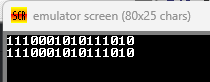
\includegraphics[width = .4\textwidth]{BIN.png}
    \captionof{figure}{Binary input \& output}
\end{center}


\clearpage
\title{Problem 4.2}
\author{}
\date{}
\maketitle

\section*{Problem Description}
Write a code to take input from user as Hexadecimal and output it as Hexadecimal.

\section*{Process}
\subsection*{Code:}

\begin{multicols}{2}{|}
    \begin{minted}[linenos,breaklines,breakanywhere]{nasm}
DATA SEGMENT
    CR EQU 0DH
    LF EQU 0AH
    CNT DB 4
DATA ENDS

CODE SEGMENT 
    ASSUME CS: CODE, DS: DATA
    
START:
    MOV AX, DATA
    MOV DS, AX
    
    XOR BX, BX
    MOV CX, 4
    
    MOV AH, 1
    INT 21H
    
INPUT:
    CMP AL, 0DH
    JE EXIT
    
    CMP AL, 39H
    JG LETTER
    
    AND AL, 0FH
    JMP SHIFT
    
LETTER:
    SUB AL, 37H    
    
SHIFT:
    SHL BX, CL
    OR BL, AL
    
    INT 21H
    
    JMP INPUT    

EXIT: 
    MOV DL, CR
    MOV AH, 2
    INT 21H
    MOV DL, LF
    INT 21H
    
PRINT:    
    MOV DL, BH
    SHR DL, 4
    ROL BX, 4
    
    CMP DL, 10 
    JL CONV_NUM
    JGE CONV_CHAR
    
CONV_NUM:
    OR DL, 30H
    MOV AH, 2
    INT 21H
    
    LOOP PRINT
    
CONV_CHAR:
    SUB DL, 9
    OR DL, 40H
    MOV AH, 2
    INT 21H

    LOOP PRINT

END1:
    MOV AH, 4CH
    INT 21H
    
CODE ENDS
ENDS START   
\end{minted}
\end{multicols}

\subsection*{Output}
\begin{center}
    \centering
    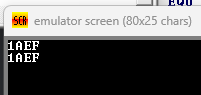
\includegraphics[width = .4\textwidth]{HEX.png}
    \captionof{figure}{Hexadecimal input \& output}
\end{center}




\section*{Keywords}
These are the new keywords learned while solving the Problems
\begin{description}
    \item[EQU] Used to declare a variable as a constant.
    \item[XOR] Used to perform Exclusive-OR operation over each bit in a byte/word with the corresponding bit in another byte/word. Used here on the same variable to clear the register.
    \item[AND] Used for adding each bit in a byte/word with the corresponding bit in another byte/word.
    \item[OR] Used to multiply each bit in a byte/word with the corresponding bit in another byte/word.
    \item[JE] Used to jump if equal/zero flag ZF = 1
    \item[SHL] Used to shift bits of a byte/word towards left and put zero(S) in LSBs.
    \item[RCL] Used to rotate bits of byte/word towards the left, i.e. MSB to CF and CF to LSB.
    \item[JC] Used to jump if carry flag CF = 1
    \item[JNC] Used to jump if no carry flag (CF = 0)
    \item[SHR] Used to shift bits of a byte/word towards the right and put zero(S) in MSBs.
    \item[ROL] Used to rotate bits of byte/word towards the left, i.e. MSB to LSB and to Carry Flag [CF].
    \item[JL] Used to jump if less than/not greater than/equal instruction satisfies.
    \item[JGE]  Used to jump if greater than/equal/not less than instruction satisfies.
\end{description}

\end{document}
